\chapter{Results}
\label{chap:results}
\section{Cytologic characterization of \emph{M. edulis} hemocyte subpopulations}
The hemolymph of \emph{Mytilus edulis} comprised a mixed population of cells differing in size, granularity, morphometrics and Wright's-Giemsa staining profiles. If the haemocytes were allowed to spread prior to fixation and staining, the diversity further expanded as cells took on a variety of shapes and/or developed cytoplasmic extensions. From these morphological criteria, a total of three distinct cell types could be identified by light microscopy.

Based on the basophilic or eosinophilic nature of their granules and other cytoplasmic contents, cytologic staining with 3 \% Wright's-Giemsa or the Hemacolor\textsuperscript{\textregistered} kit gave rise to two distinct staining profiles: basophilic and eosinophilic haemocytes. The cytoplasm of eosinophilic hemocytes (Figure \ref{fig:celltypes}, K-O) were densely packed with pink to dark purple granules of varying size and abundance. Hence, they are referred to as eosinophilic granulocytes herein. Their individual granules were usually not distinguishable in a non-spread state, but instead gave their cytoplasm an irregular pink color (Figure \ref{fig:celltypes}, K and O). These haemocytes had cell diameters in the range of 6-16 \micro m, with a mean of 9.06$\pm1.25$ \micro m. Two strikingly homogeneous features of this cell type was a small acentrically located nucleus, and a spherical to slightly oval outline in an non-spread state. With abundant pink cytoplasm making up the majority of the cells' surface area - even in the smallest specimens - the eosinophilic granulocytes could also be characterized by a low nuclear-cytoplasmic ratio (N:C ratio). If not fixed and stained before smearing - or within minutes of applying haemolymph to a glass slide - eosinophilic granulocytes were almost exclusively observed as spread cells. 

\begin{figure}[!ht]
    \centering
    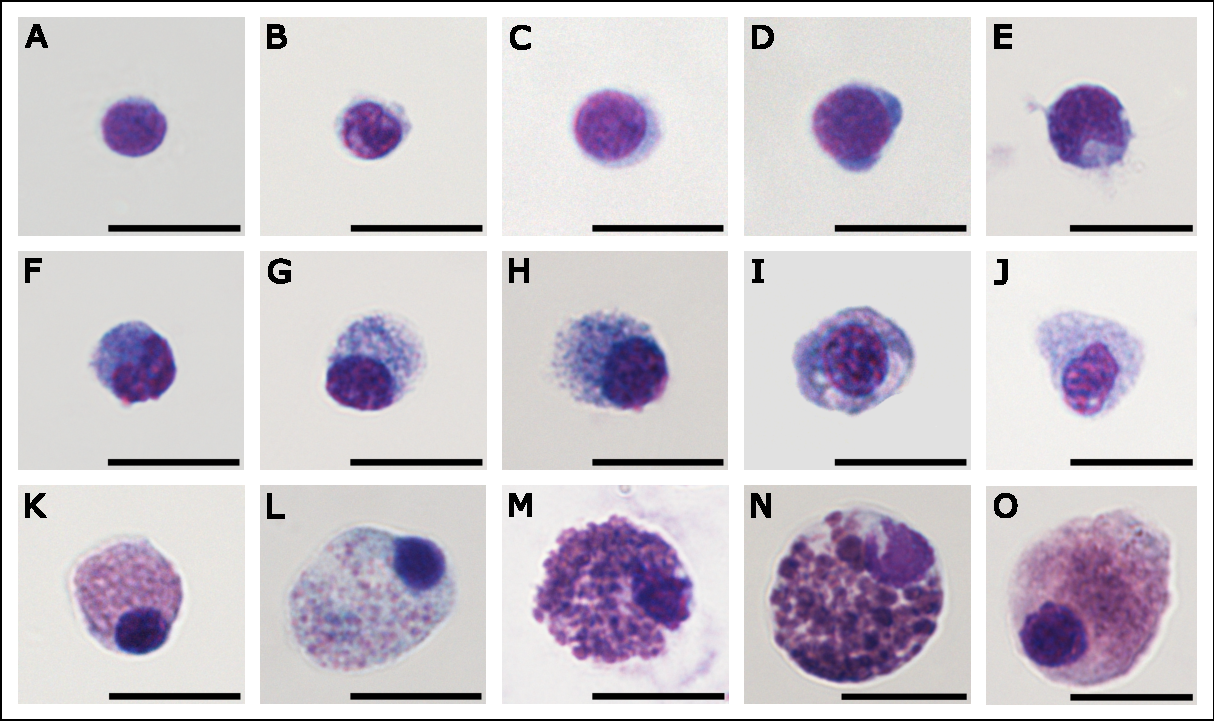
\includegraphics[width=1.0\textwidth]{figures/Anatomy/cell types brightfield updated 2.pdf}
    \caption{100$\times$ brightfield micrographs of the three haemocyte types found in the haemolymph of \emph{Mytilus edulis}, fixed and stained on glass slides with the Hemacolor\textsuperscript{\textregistered} kit before the hemocytes had time to spread notably. \textbf{(A-E)} Blast-like hyaline basophils. \textbf{(F-J)} Basophilic granulocytes. \textbf{(K-O)} Eosinophilic granulocytes. Samples were withdrawn into MPSS (1:1), scale bars = 10 \micro m.}
    \label{fig:celltypes}
\end{figure}

Compared to the eosinophilic granulocytes, the basophilic hemocytes encompassed a more heterogeneous population. Common to all of them were a larger nucleus that occupied more of the cells' total surface area (higher N:C ratio). The shape of which varied from spherical to oval, or had a distinct bean-shaped or irregular outline. But judged from the morphological criteria of cell size, granularity and N:C ratio, there were essentially two distinct subpopulations of basophilic haemocytes. One population of small hyaline blast-like haemocytes (5.63 $\pm{0.72}$ \micro m) displaying only a marginal rim of dove blue cytoplasm and no apparent cytoplasmic granules (Figure \ref{fig:celltypes}, A-E), and one population of larger haemocytes (8.07 $\pm{1.25}$ \micro m), displaying abundant basophilic cytoplasm with varying degrees of cytoplasmic granulation and vacuolation (Figure \ref{fig:celltypes}, F-J). The basophillic granules appeared much smaller than those of the eosinophilic granulocytes, and were usually not very conspicuous unless haemocytes were subjected to osmotic swelling prior to fixation and staining. Under differential interference contrast (DIC) illumination however, their granules created highly irregular surface topographies in spread cells that could be observed without such treatment. On the basis of these morphological differences, the basophilic haemocytes were subdivided into blast-like haemocytes and basophilic granulocytes herein. 

The size distributions of the three haemocyte types are shown in three kernel-smoothened density plots in Figure \ref{fig:Diameters}, together with that of the total haemocyte population. The densities have been scaled to the number of observations of each cell type, such that their relative proportions in the haemolymph of \emph{M. edulis} can be visualized. In the 20 untreated mussels examined here, the small blast-like basophils were the least abundant cell type, making up 7.9 $\pm{5.6}$ \% of the total haemocyte population. In 14 out of 20 mussels, the blast-like basophils were followed by the basophilic granulocytes, with a mean relative proportion of 40.7 $\pm{12.9}$ \%. In spite of having similar proportions to the basophilic granulocytes in several of the mussels examined here, the eosinophilic granulocytes were the most abundant cell type in the haemolymph of \emph{M edulis}, constituting 51.5 $\pm{15.3}$ \% of the total haemocyte population, on average. The relative proportions of basophilic and eosinophilic granulocytes did however vary to a large extent between individual mussels, as reflected by their standard deviations.

\begin{figure}[!ht]
    \centering
    \includegraphics[width=1.0\textwidth]{figures/Anatomy/diameters scaled density plot.pdf}
    \caption{Size distribution of \protect\dimgraybox \ small blast-like basophils (n=154), \protect\lightgraybox \ basophilic granulocytes (n=821), \protect\lysegraabox \ eosinophilic granulocytes (n=1030) and \protect\whitebox \ the total haemocyte population of \emph{Mytilus edulis} (n=2005). The diameters of 100 formaldehyde-fixed haemocytes was measured in each of 20 individual mussels, and the density was scaled to the number of observations of each cell type.}
    \label{fig:Diameters}
\end{figure}


\section{Identification of \emph{M. edulis} hemocyte subpopulations on bivariate Side scatter (SSC) and Forward scatter (FSC) dotplots}
With the BD Accuri C6 Plus benchtop flow cytometer, a maximum of three distinct hemocyte subpopulations (clusters) could be distinguished from \emph{M. edulis} hemolymph on Forwards scatter (FCS) vs. Side scatter (SSC) dotplots. These subpopulations correspond to clusters 1, 2 and 3 
 falling within the singlet gate in Figure \ref{fig:fsc_vs_ssc}, shown with SSC on both linear and logarithmic scales. The events in cluster 1 exhibit low FSC- and SSC-values relative to cluster 2 and 3, suggesting that it is populated by small and uncomplex cells. Events in both clusters 2 and 3 display higher FSC-values, but are often partially separated according to SSC.  and cluster 3 have more cells of very large diameter. is made up of cells with medium SSC- and FSC-values, with a few events having high those in gate 2 exhibit medium FSC- and SSC-values, including some events with high FSC-values, while the cells in gate 3 have high SSC-values with most of the cells

and are most likely corresponding to the small agranular cells shown in Figure [ref to Figure with cell morphology and Giemsa staining profile], with a large oval nucleus and a thin rim of basophilic staining cytoplasm. Herein we will refer to them as agranular basophils according to their Giemsa staining profile. Because of their smaller size relative to the cells in cluster 2 and 3; they are readily distinguishable with a separate peak in Coulter Counter particle-size distributions, and have cell diameters between 5.5-8 \micro m [include Figure].



\begin{figure}[!ht]
    \centering
    \includegraphics[width=1.0\textwidth]{figures/Gating strategy/lin to log.pdf}
    \caption{Hemocyte subpopulations distinguishable according to FSC vs. SSC \textbf{A} Bla bla bla.. Mention that the actual proportion was calculated counting 1000 hemocytes, and that the gates were adjusted to the true value.}
    \label{fig:fsc_vs_ssc}
\end{figure}

In some adult mussels, however, the basophilic and eosinophilic granulocyte subpopulations are partly overlapping with regard to internal complexity, i.e., SSC. Since the BD Accuri C6 Plus isn't equipped with adjustable laser gain settings, these subpopulations could not be separated further instrumentally. Thus, any attempts to gate on these subpopulations based solely on light scattering profiles, would in some mussels introduce considerable uncertainty into their relative proportions. [Find the proportion of mussels where they are not well separated, and report that number instead of saying "some" mussels here.]

Since eosinophilic granulocytes 

, and display higher density of granules (granularity), a bivariate plot of green fluorescence (518-548 nm) on log scale vs. SSC could accurately separate these subpopulations in about 1/10 of individuals (n=46, HMS data, data not shown), however the mean absolute error were [continue here]



\subsection{Eosinophilic granulocytes}


SD og absolute error

Hemocyte subpopulations and clusters

Light-scattering properties (optical characteristics)

[After the eosinophils had sedimented in the MAS buffer (sample M2 in sedimentation dataset) for 2 hours post-withdrawal (1:1), the percentage of eosinophils remaining in suspension were 72/1075 = 6.6976 \%. The 10k ToPro3 Calcein stained plot shows 7.91\%.]

\begin{figure}[!ht]
    \centering
    \includegraphics[width=1.0\textwidth]{figures/Eosin and Percoll exp/Pool II 0.75 per m.pdf}
    \caption{\textbf{Identification eosinophilic granulocytes. A} Representative light scatter profiles of... \textbf{B} }
    \label{fig:eosin_exp2}
\end{figure}

\begin{figure}[!ht]
    \centering
    \includegraphics[width=1.0\textwidth]{figures/Eosin and Percoll exp/Percoll sep for Inkscape 2.pdf}
    \caption{\textbf{Confirmation of the light scattering profiles of eosinophilic and basophilic granulocytes pre-separated by discontinuous density centrifugation. A} Light scattering profile of the 95\% pure eosinophilic fraction that separated out on top of the 43-90\% Percoll gradient interface. \textbf{B} Bla bla bla eosin separation bla bla...}
    \label{fig:Percoll-dotplots}
\end{figure}

The second round of percoll gradient separation yielded:
15\%-33\% interpface: FCM = 97\% basophils, microscopy = 96.14 \% basophils

43\%-90\% interface: FCM = 94\%, microscopy = 97.52 \%. It should be noted that these ar







